\documentclass{article}
\usepackage{../fasy-hw}

%% UPDATE these variables:
\renewcommand{\hwnum}{5}
\title{Discrete Structures, Homework \hwnum}
\author{Patrick O'Connor (Patrick OConnor (322))}
\collab{n/a}
\date{due: 19 March 2021}

\begin{document}

\maketitle

This homework assignment should be
submitted as a single PDF file both to D2L and to Gradescope.

General homework expectations:
\begin{itemize}
    \item Homework should be typeset using LaTex.
    \item Answers should be in complete sentences and proofread.
    \item You will not plagiarize.
    \item List collaborators at the start of each question using the \texttt{collab} command.
    \item Put your answers where the \texttt{todo} command currently is (and
        remove the \texttt{todo}, but not the word \texttt{Answer}).
\end{itemize}


% ============================================
% ============================================
\collab{n/a} \nextprob{Colors}
% ============================================
% ============================================

One thing that we need to consider as computer scientists is making our products
(software, technical papers) accessible to a wide range of people. When
designing GUIs or writing technical papers (e.g., journal papers or even
homework solutions), explain five things that you could do to make your
technical write-ups, website, or GUI products more accessible to people who
might be colour deficient or have Colour deficiency(or have a bad computer screen).


\paragraph{Answer}

As computer scientists in order to create more accessible products such as write-ups, websites, or GUI
we must put ourselves in the shoes of colorblind or colorweak users and reach for feedback from the end-user.
Along with this we should consider when we are first designing a product is ensuring
contrast is suitable or a color-blind web page filter option is available for
the users. As well having considering implementing text to speech buttons and keyboard access
. Another helpful implementation is to use multiple means to display your message such as using
shapes like a check-mark or a "X" to signify completion of a task or input. A
note that I remember after working with a blind CS major my freshman year is to
use heading to organize your page. The program that he used to follow along with
notes or surf the web utilized these to separate content. Lastly, providing alt-text
or descriptions for non-text content is a quick task that can assist in increasing
accessibility for those who are colorblind or colorweak. Overall at this point
many of these are industry standard at this point but I have never thought of using
these techniques for papers and I think that LaTex is a good tool for increasing
accessibility.




% ============================================
% ============================================
\collab{n/a} \nextprob{The Complete Bipartite Graph $K_{n,n}$}
% ============================================
% ============================================

How many edges does the complete bipartite graph $K_{n,n}$ have?  Make your
conjecture, then prove that it is correct.
% PAGE
Bonus: Instead, prove the more general case:
what is the number of edges in $K_{n,m}$?

\paragraph{Answer}

A complete bipartite graph $K_{n,n}$ has $n^2$ edges.

For the bonus, we consider and prove what the number of edges in $K_{n,m}$ is.

$K_{n,m}$ has $n*m$ edges.

With $K_{n,m}$ being a complete bipartite graph by the definition of bipartite graph
we know there is a union between $V_1$ and $V_2$ when $n=V_1$ and $m=V_2$.

Along with this we know that $K_{n,m}$ has exactly one edge between every
$V_1$ and $V_2$.

With this, there is only one edge for each $V_1$ and $V_2$.

Thus by the product rule we can conclude there are $V_1 * V_2 = n*m$ ways to
choose a vertex in $V_1$ and $V_2$

So if $m=n$ as in the simpler problem we have $K_{n,n} = n^2$


Definition: Bipartite Graph:  A bipartite graph is a graph in which a set of graph
vertices can be divided into two independent sets, and no two graph vertices
within the same set are adjacent. In other words, bipartite graphs can be
considered as equal to two colorable graphs. Bipartite graphs are mostly used
in modeling relationships, especially between two entire separate classes of object.
\emph{Source of definition}~\cite{techopedia}


% ============================================
% ============================================
\collab{Peyton Meeks} \nextprob{Four Colors Suffice}
% ============================================
% ============================================

Read Chapters $7$ and $8$ of \emph{Four Colors Suffice}.

\begin{enumerate}

    \item In the Four Colors Suffice book, we saw the definition of Euler's
        Formula for a finite decomposition of a Sphere or 2-plane into vertices,
        edges, and faces.  What is the other formula known as Euler's formula?

        \paragraph{Answer}

        Euler's Formula for a finite decomposition of a Sphere or 2-plane into
        vertices, edges, and faces is $V-E+F=0$

        The other formula that is known as Euler's formula is $V-E+F=2$.


    \item  Consider the following construction: Start with a solid cube.  Then, slice
        off a small region around each vertex (image you have a sharp knife, so you take
        off a tetrahedron at each corner).  How many vertices, edges, and faces are on
        the surface of this object before and after this operation? What polyhedron is this?

        \paragraph{Answer}

        The result polyhedron is a truncated hexahedron. The cube originally had 8 vertices,
        12 edges, and 6 faces. The truncated hexahedron has 24 vertices, 36 edges, and 14 faces.
        More details can be seen in the photo below.
        \begin{figure}
          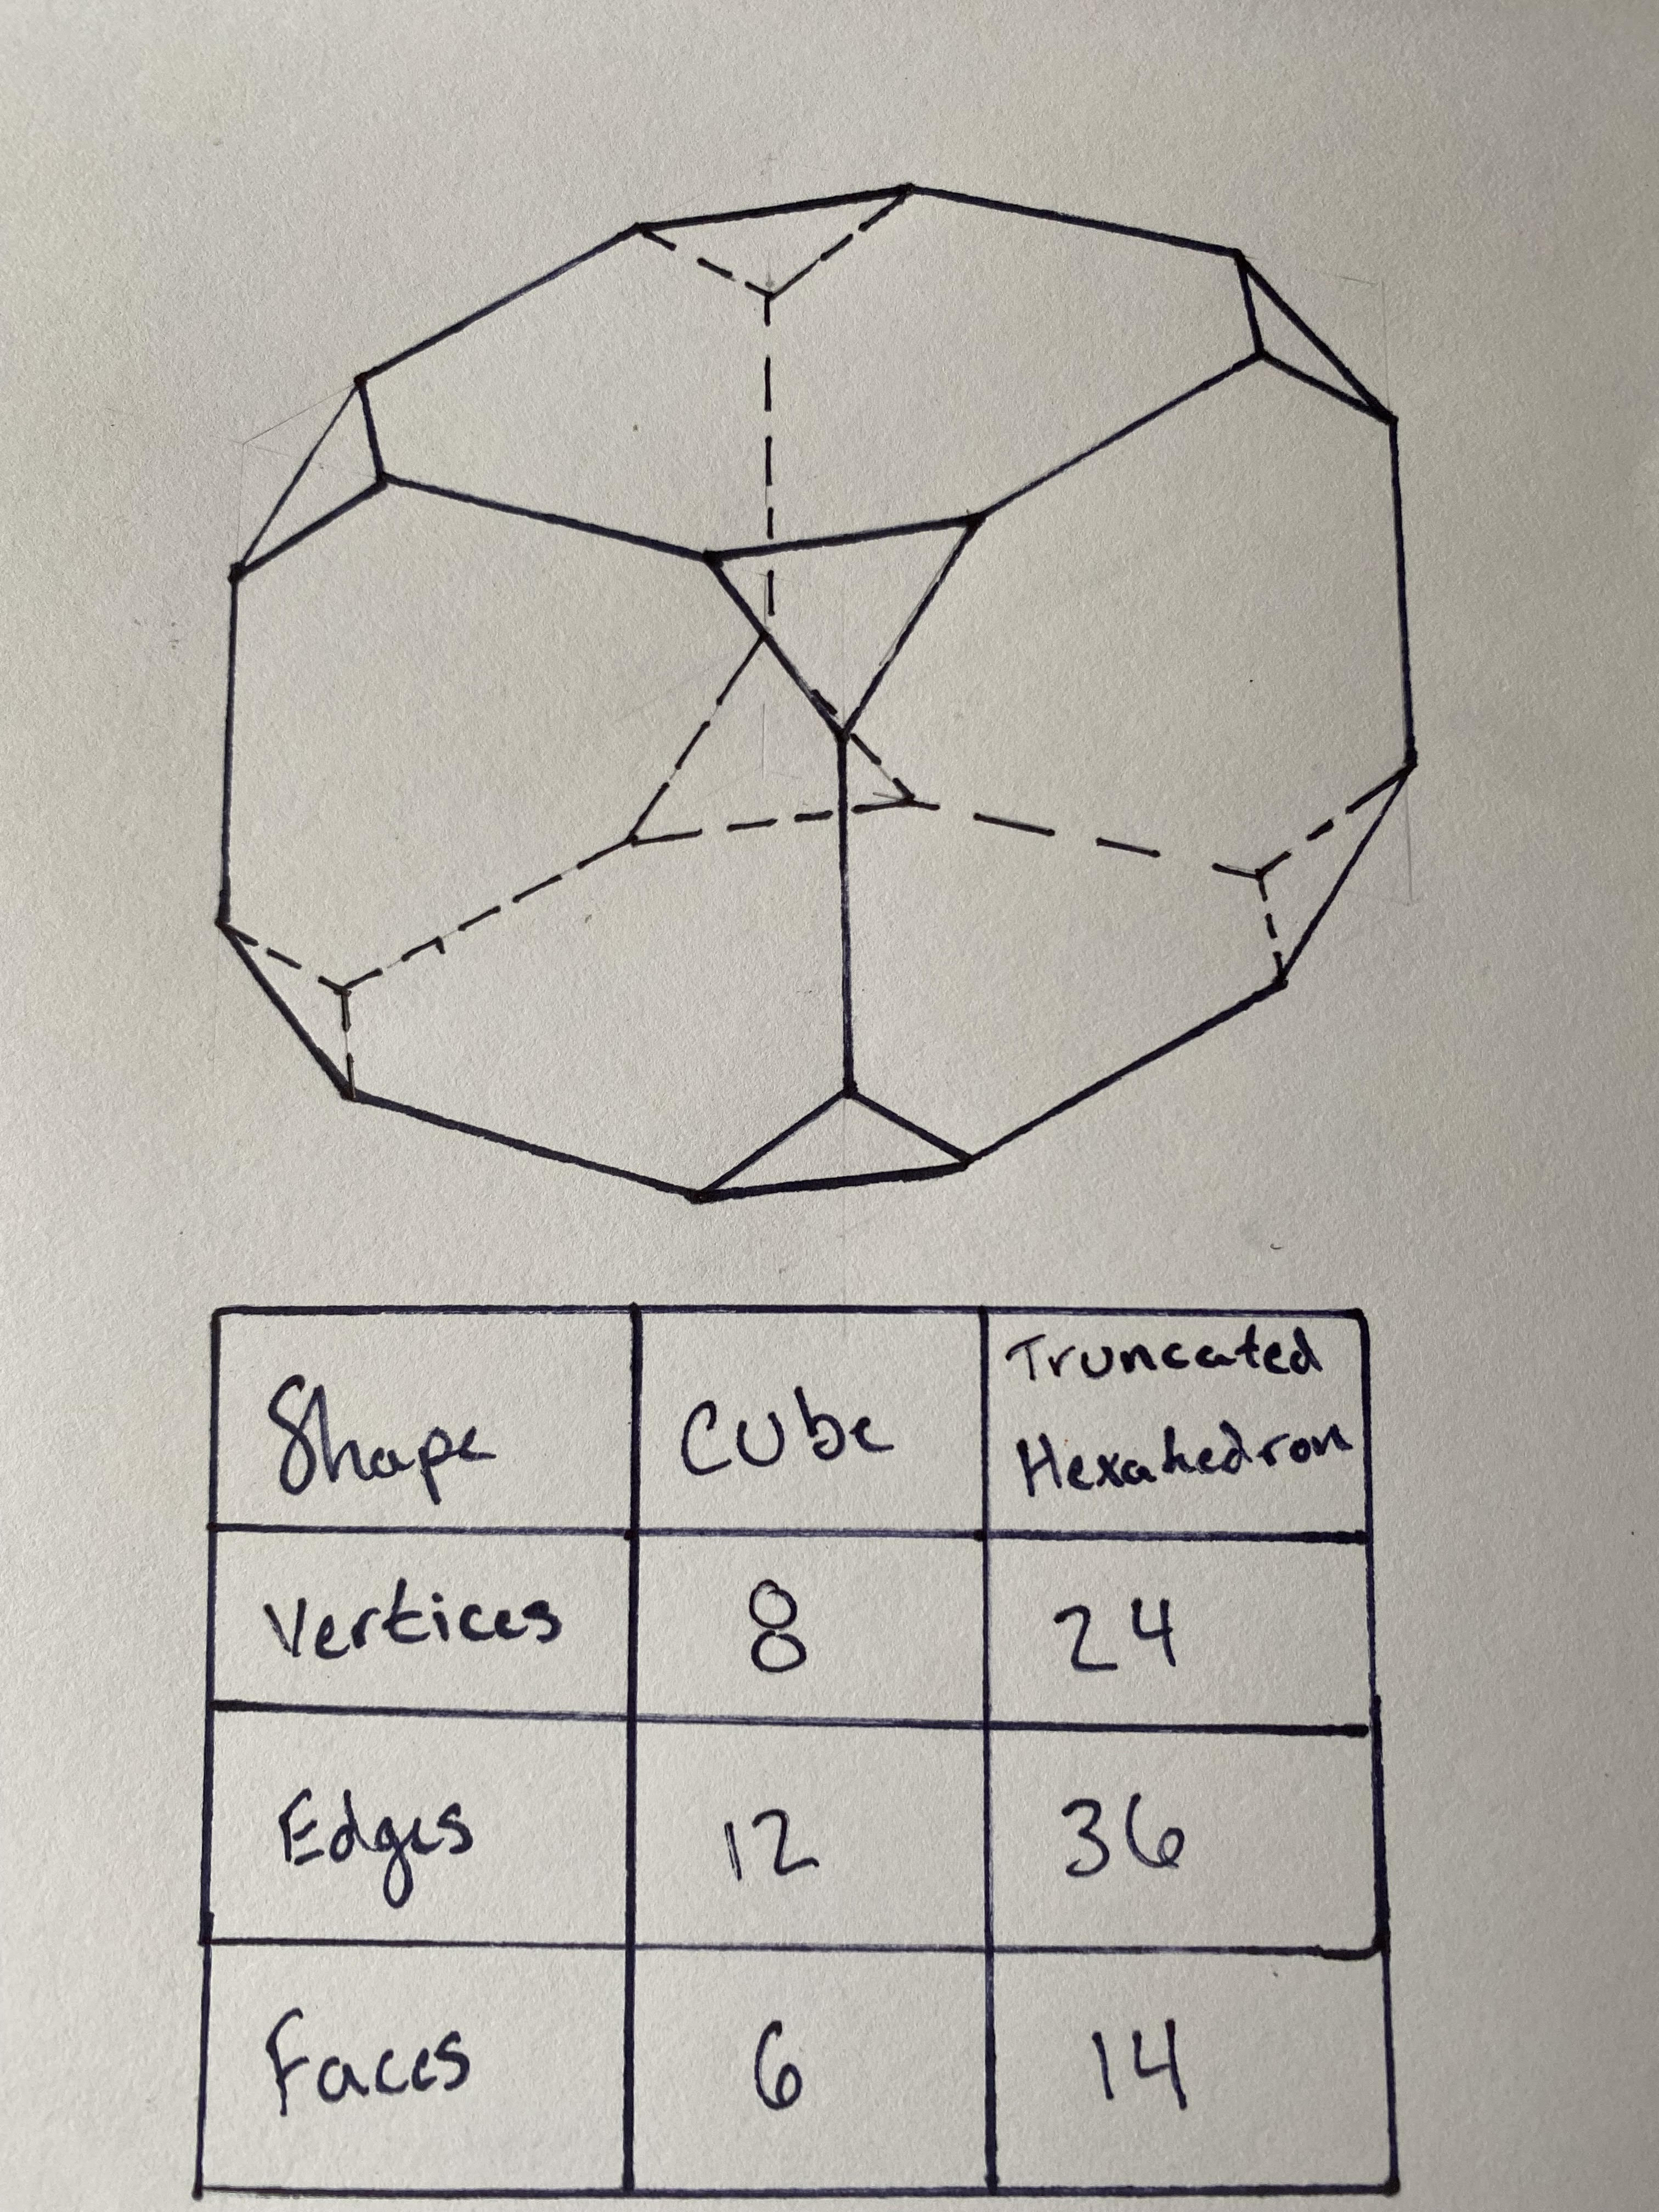
\includegraphics[width=\linewidth]{trunc-hexahedron.png}
          \caption{Solid cube with a small region sliced off at each vertex}
          \label{fig:trunc-hexahedron}
        \end{figure}
Figure \ref{fig:trunc-hexahedron} Solid cube with a small region sliced off at each vertex


    \item Draw a projection of the octahedron onto the plane such that edges only
        intersect at vertices.  Can every polyhedron be drawn in such a way?

        \paragraph{Answer}

        \begin{figure}
          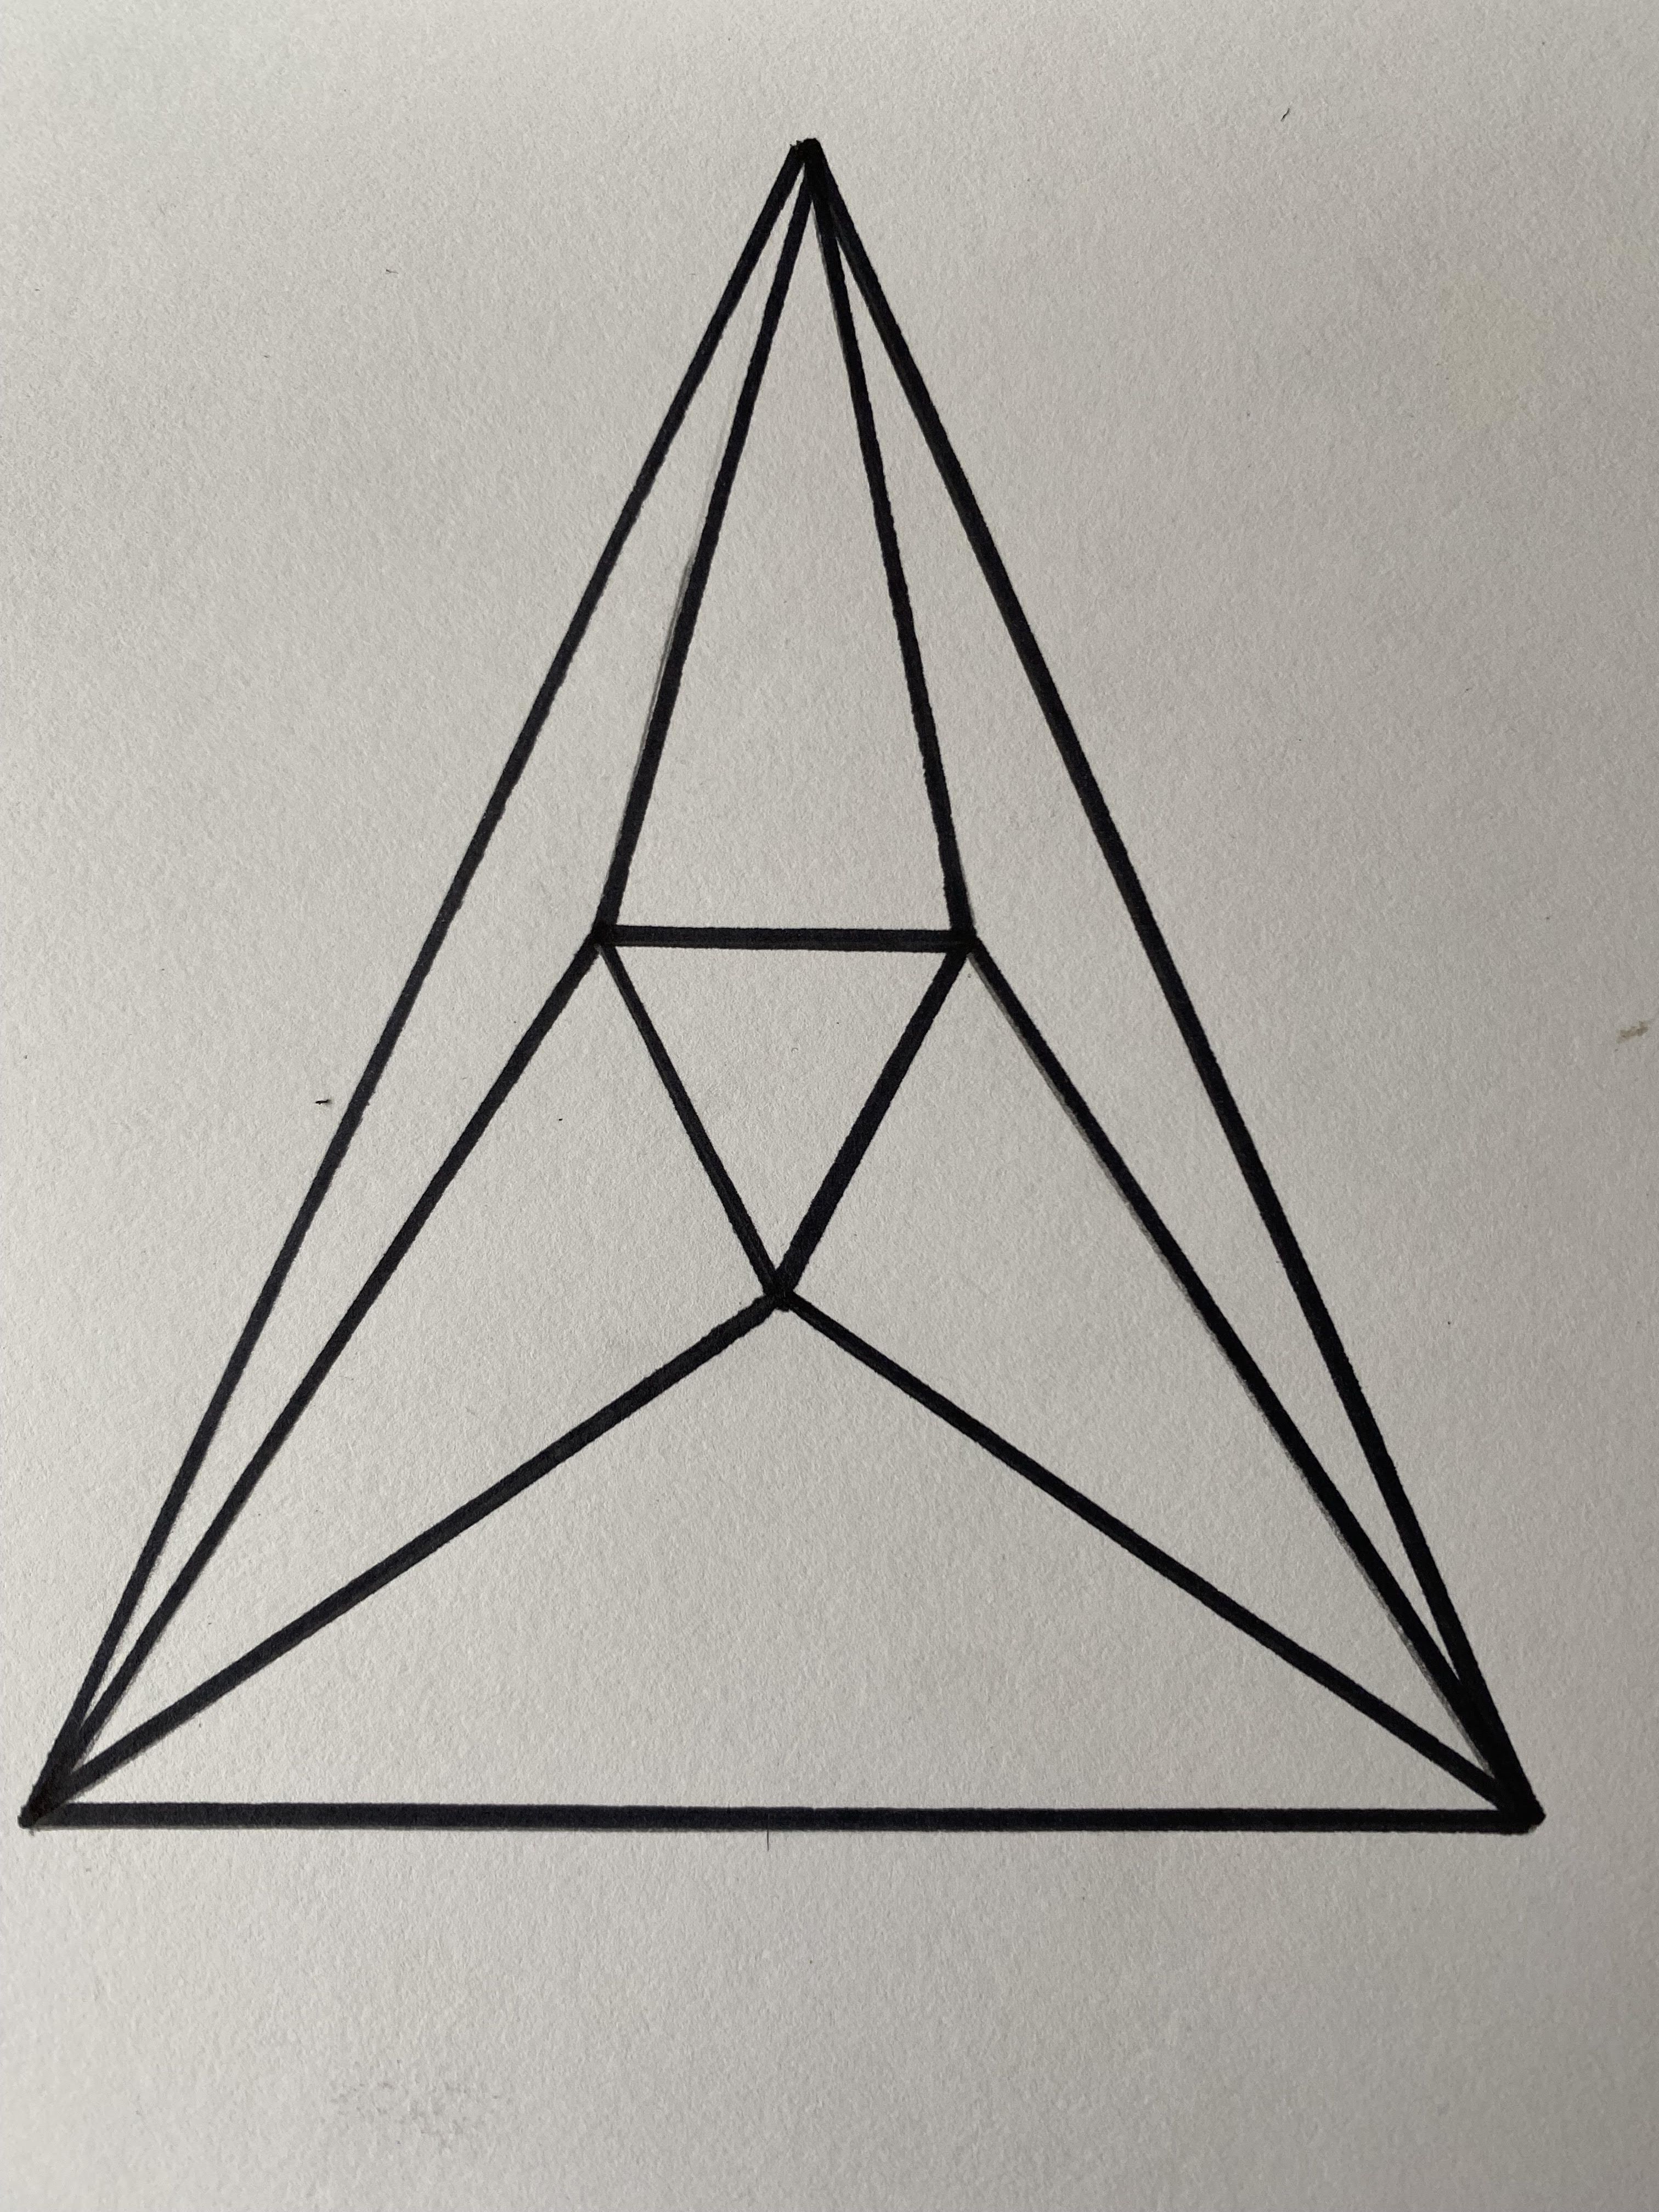
\includegraphics[width=\linewidth]{plane-octahedron.png}
          \caption{A projection of the octahedron onto the plane such that edges only
              intersect at vertices}
          \label{fig:plane-octahedron}
        \end{figure}
Figure \ref{fig:plane-octahedron} Solid cube with a small region sliced off at each vertex


\end{enumerate}

% ============================================
% ============================================
\collab{n/a}
\nextprob{Fran Allen}
% ============================================
% ============================================

Write a short (1-2 paragraph) biography of Fran Allen.
\textbf{In your own words}, describe who they are and why they are important in
the history of computer science.

If you use external resources, please provide
proper citations. If you do not use external sources, please write ``I did not
use any sources to write this biography'' as the last sentence of the
biography.

\paragraph{Answer}
Frances E. Allen is an American computer scientist that grew up on a farm in Peru,
New York. Growing up in a small town she had been home schooled by a neighbor.
Later attending The New York State College for Teachers for a bachelors of science
degree in mathematics. After graduating she went back to her home town and began
educating the youth in mathematics. After a couple years she went back to school
at the University of Michigan for a master of science in mathematics.

After graduating, she left the education sector and joined the IBM team. Although
leaving the education sector technically she was hired to teach the existing
staff scientists about a new programming language named FORTRAN. At the time FORTRAN
had been released just two months before. After a couple years of teaching and
diving into the FORTRAN compiler source code Allen progressed to working on
compilers for IBM supercomputers. This compiler work is were she made the
largest amount of progress in the computing world and subsequently was awarded
a A.M. Turing Award. Allen's focus throughout her career was on compiler optimization.
Her work in compilers was to decrease the size of the bridge between how computers
communicate and humans communicate. Along with this expansive work within compilers
Frances Allen spoke at a conferences across the world inspiring many young women
to go into the field of computer science.
\emph{Wikipedia}~\cite{wikipedia}
\emph{Britannica}~\cite{britannica}

% %% ... the bibliography
 \newpage
 \bibliographystyle{acm}
 \bibliography{biblio}

\end{document}
